\clearpage

\section{Error Vector Magnitude}
\label{sec:error_vector_magnitude}
\begin{refsection}

\begin{tcolorbox}	
\begin{tabular}{p{2.75cm} p{0.2cm} p{10.5cm}} 	
\textbf{Header File}    &:& error\_vector\_magnitude\_*.h \\
\textbf{Source File}    &:& error\_vector\_magnitude\_*.cpp \\
\textbf{Version}        &:& 20190114 (Daniel Pereira)
\end{tabular}
\end{tcolorbox}

\subsection*{Input Parameters}

\begin{table}[H]
\centering
\begin{tabular}{|l|l|l|}
\hline
Name               & Type           & Default Value     \\ \hline
referenceAmplitude & double         & 1.0              \\ \hline
m                  & integer        & 0                 \\ \hline
midRepType         & enum           & Cumulative \\ \hline
\end{tabular}
\end{table}


\subsection*{Methods}

\begin{itemize}
  \item ErrorVectorMagnitude(vector<Signal *> \&InputSig, vector<Signal *> \&OutputSig) :Block(InputSig,OutputSig)\{\};
  \item void initialize(void);
  \item bool runBlock(void);
  \item void setMidReportSize(int M) \{ m = M; \}
  \item void setMidReportType(MidReportType mrt) \{ midRepType = mrt; \}
  \item void setReferenceAmplitude(double rAmplitude) \{ referenceAmplitude = rAmplitude; \}
	
\end{itemize}




\subsection*{Input Signals}

\textbf{Number}: 1\\
\textbf{Type}: Complex (DiscreteTimeContinuousAmplitude)


\subsection*{Output Signals}

\textbf{Number}: 1\\
\textbf{Type}: Complex (DiscreteTimeContinuousAmplitude)

\subsection*{Functional Description}

This block accepts one binary string and outputs copy of the input binary string. This block also outputs .txt files with a report of the estimated Error Vector Magnitude (EVM), $\widehat{EVM}$.
\par
The block allows for mid-reports to be generated, the number of bits between reports is customizable, if it is set to 0 then the block will only output the final report. This block can operate mid-reports using CUMULATIVE mode, in which $\widehat{EVM}$ is calculated taking into account all received points, or in a RESET mode, in which $\widehat{EVM}$ is computed from only the points after the previous mid-report.

\subsection*{Theoretical Description}

The $\widehat{\text{EVM}}$ is obtained by evaluating the relation between the magnitude of the error vector $\vec{e}_v$ and the magnitude of the vector of the ideal symbol position $\vec{ref}_v$. This process is presented visually in Figure~\ref{fig:EVM} and is described by
\begin{equation}
\widehat{\text{EVM}}=100\sqrt{\frac{|\vec{e}_v|}{|\vec{ref}_v|}}=100\sqrt{\frac{|\vec{m}_v-\vec{ref}_v|}{|\vec{ref}_v|}}.
\end{equation}

\begin{figure}[h]
\centering
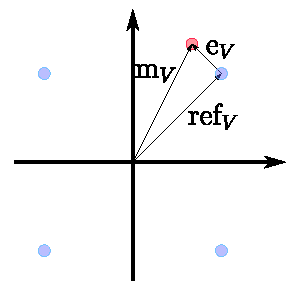
\includegraphics{evm.pdf}
\caption{Visual representation of the EVM method in a QPSK constellation. The igual constellation points are presented in blue, while an example for the actual measured symbol is presented in red.}
\label{fig:EVM}
\end{figure}


% bibliographic references for the section ----------------------------
\clearpage
\printbibliography[heading=subbibliography]
\end{refsection}
\addcontentsline{toc}{subsection}{Bibliography}
\cleardoublepage
% --------------------------------------------------------------------- 